\apendice{Especificación de Requisitos}

\section{Introducción}
Este apéndice detalla la especificación de requisitos del sistema AgroSkopos. Se enumeran los objetivos generales que motivan el desarrollo, seguidos de un catálogo exhaustivo de los requisitos funcionales organizados por módulos. Finalmente, se detalla la especificación de los casos de uso principales, describiendo el flujo de interacción entre los distintos actores (Usuario, Operador, Administrador) y el sistema.

\section{Objetivos generales}
El principal objetivo que se planteó para este proyecto era desarrollar una solución que permita a una empresa o explotación agrícola manejar y gestionar un robot agrícola de forma centralizada y remota. Para lograr este fin, se han definido los siguientes objetivos secundarios:
\begin{itemize}
    \item Desarrollar una plataforma centralizada y segura para la gestión de usuarios y roles dentro del entorno empresarial.
    \item Proveer capacidades de monitorización y telemetría en tiempo real, ofreciendo datos críticos del estado del robot y del terreno.
    \item Implementar un sistema de control bidireccional que permita la operación manual remota y la navegación autónoma.
    \item Facilitar la planificación y ejecución de misiones agrícolas autónomas mediante herramientas de \textit{geofencing}.
\end{itemize}

\section{Catálogo de requisitos}

\subsection{Módulo de Autenticación y Seguridad}
\begin{itemize}
    \item \textbf{RF-1.1 (Inicio de Sesión):} El sistema debe permitir a los empleados iniciar sesión introduciendo su nombre de usuario y contraseña.
    \item \textbf{RF-1.2 (Cierre de Sesión):} El sistema debe permitir a los usuarios cerrar su sesión de forma segura, invalidando el acceso.
    \item \textbf{RF-1.3 (Restricción de Registro):} El sistema no debe permitir el auto-registro público de usuarios. La creación de cuentas es exclusiva de la administración.
    \item \textbf{RF-1.4 (Gestión de Perfil Propio):} El sistema debe permitir a cualquier empleado autenticado modificar su contraseña.
\end{itemize}

\subsection{Módulo de Administración de Cuentas}
\begin{itemize}
    \item \textbf{RF-2.1 (Creación de Empleados):} El sistema debe permitir al Administrador dar de alta nuevas cuentas de empleados en la plataforma.
    \item \textbf{RF-2.2 (Asignación de Roles):} El sistema debe permitir al Administrador asignar y modificar el nivel de privilegio de un usuario (Admin, Operador, Usuario).
    \item \textbf{RF-2.3 (Baja de Empleados):} El sistema debe permitir al Administrador deshabilitar o eliminar cuentas de empleados.
    \item \textbf{RF-2.4 (Listado de Usuarios):} El sistema debe proporcionar al Administrador una vista con todos los usuarios registrados y su rol actual.
\end{itemize}

\subsection{Módulo de Monitorización y Telemetría}
\begin{itemize}
    \item \textbf{RF-3.1 (Posicionamiento GPS):} El sistema debe mostrar en un mapa interactivo la ubicación exacta del robot actualizada en tiempo real.
    \item \textbf{RF-3.2 (Estado de Energía):} El sistema debe mostrar el porcentaje de batería, si está cargando o descargando, y mostrar información sobre la potencia instantánea de generación solar.
    \item \textbf{RF-3.3 (Estado General):} El sistema debe informar sobre la actividad actual del robot (Ej: En espera, Trabajando, Regresando a base).
    \item \textbf{RF-3.4 (Lecturas Agronómicas):} El sistema debe mostrar al instante los valores simulados recogidos por los sensores del suelo (Humedad, Temperatura, pH, N-P-K y Radiación).
\end{itemize}

\subsection{Módulo de Operación y Control Directo}
\begin{itemize}
    \item \textbf{RF-4.1 (Cambio de Modo):} El sistema debe permitir al Operador alternar entre los modos de funcionamiento del robot (Manual, Autónomo, Navegación).
    \item \textbf{RF-4.2 (Control Manual Remoto):} El sistema debe proporcionar un sistema de control mediante los botones de dirección de la interfaz o las flechas del teclado para conducir el robot en modo Manual.
    \item \textbf{RF-4.3 (Control de Velocidad):} El sistema debe permitir al Operador modificar la velocidad de desplazamiento del robot en tiempo real.
    \item \textbf{RF-4.4 (Navegación por \textit{waypoints}):} El sistema debe permitir encolar puntos en el mapa para que el robot navegue hacia ellos.
    \item \textbf{RF-4.5 (Pausa Rápida):} El sistema debe permitir pausar temporalmente cualquier movimiento del robot y poder reanudarlo.
    \item \textbf{RF-4.6 (Parada de Emergencia):} El sistema debe disponer de un control de emergencia que aborte inmediatamente la misión y detenga los motores.
    \item \textbf{RF-4.7 (Transmisión de Vídeo):} El sistema debe integrar un flujo de vídeo en tiempo real para facilitar la supervisión visual durante la operación y control del robot.
\end{itemize}

\subsection{Módulo de Gestión de Misiones Autónomas}
\begin{itemize}
    \item \textbf{RF-5.1 (Gestión CRUD de Misiones):} El sistema debe permitir al Operador crear nuevas misiones, modificarlas, eliminarlas y consultar su histórico.
    \item \textbf{RF-5.2 (Dibujo de Área de Trabajo):} El sistema debe proveer herramientas para dibujar un polígono que delimite la parcela de trabajo.
    \item \textbf{RF-5.3 (Zonas de Exclusión):} El sistema debe permitir dibujar huecos o zonas de exclusión dentro del área principal donde el robot no deberá entrar.
    \item \textbf{RF-5.4 (Configuración de Parámetros de Ruta):} El sistema debe permitir ajustar el ancho entre pasada y pasada para la generación de la ruta en zig-zag.
    \item \textbf{RF-5.5 (Selección de Sensores):} El sistema debe permitir elegir qué datos se van a recoger durante la misión (ej. solo humedad, o reconocimiento rápido sin recogida de datos).
    \item \textbf{RF-5.6 (Umbral de Batería Inicial):} El sistema debe permitir establecer una batería mínima requerida para autorizar el inicio de la misión.
    \item \textbf{RF-5.7 (Lanzamiento de Misiones):} El sistema debe permitir iniciar la ejecución autónoma de una misión previamente configurada.
\end{itemize}

\subsection{Módulo de Lógica Autónoma de Seguridad}
\begin{itemize}
    \item \textbf{RF-6.1 (Retorno Inteligente a Base):} El robot debe calcular continuamente la distancia hasta la estación de carga y retornar de forma autónoma cuando determine que la batería es estrictamente la necesaria para el trayecto de vuelta.
    \item \textbf{RF-6.2 (Reanudación Post-Carga):} El sistema debe volver al punto de interrupción para continuar la misión una vez recargado al 100\%.
    \item \textbf{RF-6.3 (Reposo Seguro):} El sistema debe enviar automáticamente al robot a la base de carga si permanece inactivo durante un periodo prolongado.
\end{itemize}

\subsection{Módulo de Análisis de Datos Agronómicos}
\begin{itemize}
    \item \textbf{RF-7.1 (Exportación de Datos):} El sistema debe permitir la exportación de los datos recogidos y análisis mostrados a formatos estándar (PDF y CSV).
    \item \textbf{RF-7.2 (Filtros Temporales y por Misión):} El sistema debe incluir un calendario para filtrar los datos mostrados indicando fecha, hora y misión específica.
    \item \textbf{RF-7.3 (Visualización de Gráficas):} El sistema debe generar gráficas temporales con un único parámetro o gráficas comparativas cruzando dos variables agronómicas.
    \item \textbf{RF-7.4 (Visualización Tabular):} El sistema debe presentar una tabla detallada con todos los datos crudos recogidos, incluyendo la hora exacta y la localización de la muestra.
    \item \textbf{RF-7.5 (Geolocalización de Muestras):} El sistema debe permitir al usuario conocer la localización en el mapa de cada dato individual recogido.
    \item \textbf{RF-7.6 (Mapa de Puntos y Medias por Zona):} El sistema debe mostrar un mapa con los puntos donde se tomaron medidas, permitiendo agrupar/filtrar por zona para visualizar la media aritmética de los valores recogidos en dicha área.
\end{itemize}

\subsection{Módulo de Usabilidad e Integración}
\begin{itemize}
    \item \textbf{RF-8.1 (Internacionalización):} El sistema debe permitir al usuario cambiar el idioma de la interfaz gráfica en tiempo real, soportando al menos los idiomas español, inglés y portugués.
    \item \textbf{RF-8.2 (Aplicación Web Progresiva):} El sistema debe ofrecer la capacidad de ser instalado como una aplicación nativa en dispositivos móviles (PWA) para facilitar su operabilidad a pie de campo.
    \item \textbf{RF-8.3 (Documentación Interactiva de API):} El servidor debe exponer una interfaz web donde los desarrolladores y administradores puedan explorar y probar interactivamente los \textit{endpoints} del sistema (Swagger).
\end{itemize}

\subsection{Módulo de Notificaciones y Reportes}
\begin{itemize}
    \item \textbf{RF-9.1 (Envío de Credenciales Autogeneradas):} El sistema debe enviar automáticamente un correo electrónico de bienvenida con la contraseña autogenerada cuando el Administrador da de alta a un nuevo empleado.
    \item \textbf{RF-9.2 (Sistema de Soporte por Tickets):} El sistema debe permitir a los usuarios reportar problemas o incidencias técnicas mediante la generación de un ticket que se enviará automáticamente por correo electrónico al equipo responsable.
    \item \textbf{RF-9.3 (Distribución de Reportes):} El sistema debe permitir tanto la descarga local (en formatos PDF y CSV) de los análisis agronómicos, como su envío directo por correo electrónico a la dirección solicitada.
\end{itemize}

\subsection{Requisitos No Funcionales}
\begin{itemize}
    \item \textbf{RNF-1 (Rendimiento y Latencia):} El sistema de telemetría y control remoto debe operar con una latencia mínima, garantizando una respuesta fluida a los comandos manuales y a la recepción de datos en tiempo real.
    \item \textbf{RNF-2 (Escalabilidad de Sistema):} La arquitectura del servidor y la base de datos deben permitir la escalabilidad para gestionar un alto volumen de datos históricos y soportar el control de múltiples robots de forma simultánea en el futuro.
    \item \textbf{RNF-3 (Portabilidad y Despliegue):} El sistema debe estar estructurado en contenedores virtuales que aíslen los diferentes servicios, garantizando un despliegue rápido y reproducible en cualquier entorno o servidor.
    \item \textbf{RNF-4 (Protección de Red y API):} Las interfaces de comunicación deben incorporar mecanismos robustos de seguridad (como limitación de tasa de peticiones, control de origen cruzado y fortificación de cabeceras) para prevenir abusos y ataques externos.
    \item \textbf{RNF-5 (Integridad de Transacciones):} Las operaciones críticas que requieran múltiples escrituras deben estar protegidas mediante transacciones de base de datos para asegurar que no quede información corrupta o huérfana en caso de error.
    \item \textbf{RNF-6 (Usabilidad Responsiva):} La interfaz de usuario debe ser completamente adaptativa y ofrecer notificaciones claras, posibilitando su uso seguro e intuitivo tanto en monitores de escritorio como en dispositivos táctiles en el campo.
    \item \textbf{RNF-7 (Calidad de Código y Análisis Estático):} El código fuente debe someterse a análisis estático continuo para detectar vulnerabilidades, \textit{code smells} y garantizar el cumplimiento de métricas de calidad predefinidas.
    \item \textbf{RNF-8 (Integración Continua):} La adición de nuevas características debe estar respaldada por tuberías de integración continua (CI) que automaticen la validación del código antes de ser desplegado.
    \item \textbf{RNF-9 (Fiabilidad y Cobertura de Pruebas):} Los módulos deben contar con una batería de pruebas unitarias y de integración automatizadas para prevenir regresiones y asegurar su correcto funcionamiento.
    \item \textbf{RNF-10 (Validación Estricta de Datos):} El sistema debe implementar mecanismos rigurosos de validación de esquemas en todas las entradas de datos para prevenir errores de tipo y fallos en tiempo de ejecución.
    \item \textbf{RNF-11 (Documentación de Código Autogenerada):} El código fuente debe estar debidamente documentado mediante un formato estandarizado (como JSDoc) que permita la generación automática y actualización continua de la documentación técnica.
    \item \textbf{RNF-12 (Pruebas de Carga y Estrés):} El servidor debe soportar picos de peticiones y tráfico intensivo de telemetría sin degradación notable. La resistencia debe validarse mediante inyección de carga con herramientas como k6.
    \item \textbf{RNF-13 (Despliegue Híbrido Cloud):} El sistema debe desplegar la API REST y la base de datos en servidores virtuales (como Microsoft Azure) y el cliente en una red de entrega global estática (como Vercel) para optimizar la latencia.
\end{itemize}

\section{Especificación de requisitos}
A continuación se detallan los casos de uso principales identificados para el sistema AgroSkopos.

Antes de detallar las interacciones de cada caso de uso, es necesario definir los \textbf{Actores del Sistema}. El sistema implementa un modelo de permisos jerárquico e incremental basado en los siguientes roles:
\begin{itemize}
    \item \textbf{Usuario:} Dispone de acceso de solo lectura. Puede acceder a la plataforma web para monitorizar la telemetría en tiempo real, visualizar la posición del robot en el mapa y consultar el histórico de datos y gráficas agronómicas. No tiene permisos para alterar el estado del sistema ni enviar comandos al robot.
    \item \textbf{Operador:} Hereda todos los permisos de visualización del perfil \textit{Usuario}. Además, está capacitado para tomar el control activo del vehículo. Puede conducir el robot en modo manual, dibujar áreas de trabajo, configurar parámetros y lanzar misiones autónomas.
    \item \textbf{Administrador (Admin):} Posee el control total del sistema. Hereda las capacidades operativas del \textit{Operador} y añade privilegios exclusivos de gestión interna, como la creación, modificación y eliminación de cuentas de empleados, así como la asignación de roles.
\end{itemize}

Para ilustrar de manera general las interacciones de estos actores, la figura \ref{fig:img/apendice_B/diagrama_casos_uso.png} muestra el diagrama de casos de uso completo del sistema.

\begin{figure}[!h]
    \centering
    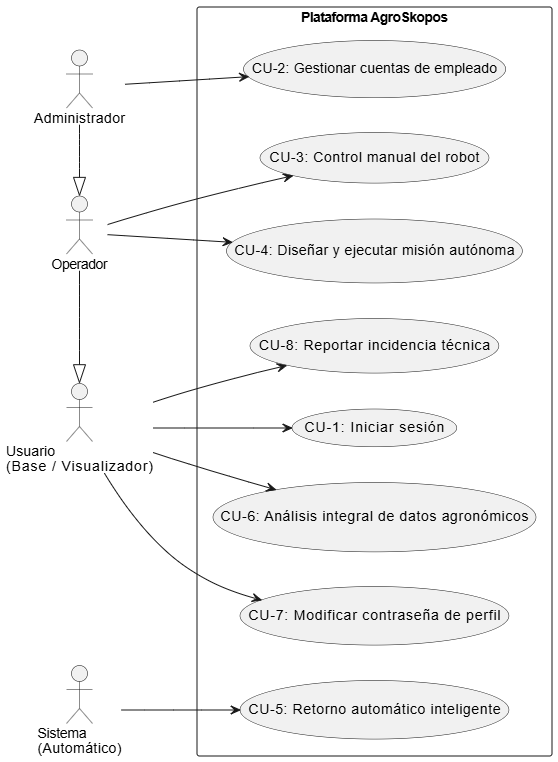
\includegraphics[width=1\textwidth,height=0.9\textheight,keepaspectratio]{img/apendice_B/diagrama_casos_uso.png}
    \caption{Diagrama General de Casos de Uso del Sistema}\label{fig:img/apendice_B/diagrama_casos_uso.png}
\end{figure}
\clearpage

% CU-1 Iniciar Sesión
\begin{table}[H]
	\centering
	\begin{tabularx}{\linewidth}{ p{0.21\columnwidth} p{0.71\columnwidth} }
		\toprule
		\textbf{CU-1}    & \textbf{Iniciar sesión}\\
		\toprule
		\textbf{Versión}              & 1.0    \\
		\textbf{Autor}                & Andrés Vera Cachoo \\
		\textbf{Actores}              & Usuario, Operador, Administrador \\
		\textbf{Requisitos asociados} & RF-1.1 \\
		\textbf{Descripción}          & Permite a un empleado acceder a la plataforma mediante sus credenciales. \\
		\textbf{Precondición}         & El usuario debe estar registrado por un Administrador y disponer de credenciales válidas. \\
		\textbf{Acciones}             &
		\begin{enumerate}
			\def\labelenumi{\arabic{enumi}.}
			\tightlist
			\item El usuario accede a la página de inicio de sesión.
			\item El sistema solicita correo electrónico y contraseña.
			\item El usuario introduce sus datos y pulsa el botón de acceso.
            \item El sistema valida las credenciales y devuelve un \textit{token} de acceso (\textbf{JWT}).
            \item El sistema redirige al usuario a la vista principal (\textit{dashboard}).
		\end{enumerate}\\
		\textbf{Postcondición}        & El usuario queda autenticado y tiene acceso a las funciones permitidas por su rol. \\
		\textbf{Excepciones}          & Credenciales incorrectas: El sistema deniega el acceso y muestra un mensaje de error. \\
		\textbf{Importancia}          & Alta \\
		\bottomrule
	\end{tabularx}
	\caption{CU-1 Iniciar sesión.}
\end{table}

% CU-2 Gestión de usuarios
\begin{table}[H]
	\centering
	\begin{tabularx}{\linewidth}{ p{0.21\columnwidth} p{0.71\columnwidth} }
		\toprule
		\textbf{CU-2}    & \textbf{Gestionar cuentas de empleado}\\
		\toprule
		\textbf{Versión}              & 1.0    \\
		\textbf{Autor}                & Andrés Vera Cachoo \\
		\textbf{Actores}              & Administrador \\
		\textbf{Requisitos asociados} & RF-2.1, RF-2.2, RF-2.3, RF-2.4 \\
		\textbf{Descripción}          & Permite al Administrador dar de alta, modificar roles o eliminar empleados del sistema. \\
		\textbf{Precondición}         & El usuario debe estar autenticado y tener el rol \textit{Admin}. \\
		\textbf{Acciones}             &
		\begin{enumerate}
			\def\labelenumi{\arabic{enumi}.}
			\tightlist
			\item El Administrador navega a la sección de "Gestión de Usuarios".
			\item El sistema muestra un listado con los usuarios actuales.
			\item El Administrador selecciona crear un nuevo usuario o editar uno existente.
            \item El Administrador introduce/modifica los datos (nombre, correo, rol) y guarda.
            \item El sistema actualiza la base de datos y refleja los cambios en el listado.
            \item (Solo si es un alta nueva) El sistema envía un correo electrónico automatizado al empleado con sus credenciales iniciales.
		\end{enumerate}\\
		\textbf{Postcondición}        & Las credenciales y privilegios del usuario afectado se actualizan y el empleado recibe su notificación de alta. \\
		\textbf{Excepciones}          & Correo duplicado al crear usuario: El sistema informa de que la cuenta ya existe. Fallo en el servidor SMTP: El usuario se crea, pero se informa de que el correo no pudo enviarse. \\
		\textbf{Importancia}          & Alta \\
		\bottomrule
	\end{tabularx}
	\caption{CU-2 Gestionar cuentas de empleado.}
\end{table}

% CU-3 Control manual
\begin{table}[H]
	\centering
	\begin{tabularx}{\linewidth}{ p{0.21\columnwidth} p{0.71\columnwidth} }
		\toprule
		\textbf{CU-3}    & \textbf{Control manual del robot}\\
		\toprule
		\textbf{Versión}              & 1.0    \\
		\textbf{Autor}                & Andrés Vera Cachoo \\
		\textbf{Actores}              & Operador, Administrador \\
		\textbf{Requisitos asociados} & RF-4.1, RF-4.2, RF-4.3 \\
		\textbf{Descripción}          & El Operador toma el control directo del movimiento usando botones en pantalla o teclado, pudiendo regular la velocidad. \\
		\textbf{Precondición}         & El usuario debe tener rol \textit{Operador} o \textit{Admin}. El robot debe tener conexión y batería suficiente. \\
		\textbf{Acciones}             &
		\begin{enumerate}
			\def\labelenumi{\arabic{enumi}.}
			\tightlist
			\item El Operador establece el modo de funcionamiento del robot a "Manual".
            \item El Operador ajusta el nivel de velocidad deseado.
			\item El Operador presiona las flechas de dirección en la interfaz o su teclado.
			\item El sistema envía vectores de velocidad y dirección mediante \textit{WebSockets} al simulador/robot.
            \item El robot procesa el movimiento y actualiza su posición en el mapa interactivo.
		\end{enumerate}\\
		\textbf{Postcondición}        & El robot se desplaza según las indicaciones del Operador. \\
		\textbf{Excepciones}          & Pérdida de conexión: El robot se detiene automáticamente por seguridad. \\
		\textbf{Importancia}          & Alta \\
		\bottomrule
	\end{tabularx}
	\caption{CU-3 Control manual del robot.}
\end{table}

% CU-4 Crear Mision
\begin{table}[H]
	\centering
	\begin{tabularx}{\linewidth}{ p{0.21\columnwidth} p{0.71\columnwidth} }
		\toprule
		\textbf{CU-4}    & \textbf{Diseñar y ejecutar misión autónoma}\\
		\toprule
		\textbf{Versión}              & 1.0    \\
		\textbf{Autor}                & Andrés Vera Cachoo \\
		\textbf{Actores}              & Operador, Administrador \\
		\textbf{Requisitos asociados} & RF-5.2, RF-5.3, RF-5.4, RF-5.5 \\
		\textbf{Descripción}          & El Operador planifica al detalle una ruta de barrido definiendo parcelas, huecos y sensores a activar. \\
		\textbf{Precondición}         & Rol \textit{Operador} o \textit{Admin}. El robot está en espera y supera el umbral mínimo de batería. \\
		\textbf{Acciones}             &
		\begin{enumerate}
			\def\labelenumi{\arabic{enumi}.}
			\tightlist
			\item El Operador accede a la herramienta de Misiones y dibuja el polígono externo de la parcela en el mapa.
			\item El Operador delimita sub-polígonos como "zonas de exclusión" dentro de la parcela.
            \item El Operador configura el espaciado de las pasadas en zig-zag y los sensores a utilizar.
			\item El sistema calcula una ruta óptima evitando los huecos marcados.
            \item El Operador hace clic en "Iniciar Misión". El robot cambia a modo "Autónomo" y sigue la trayectoria.
		\end{enumerate}\\
		\textbf{Postcondición}        & La misión se registra en el historial como "En curso" y el robot opera recolectando los datos seleccionados. \\
		\textbf{Excepciones}          & Batería inferior al mínimo de seguridad configurado: El sistema rechaza iniciar la misión. \\
		\textbf{Importancia}          & Muy Alta \\
		\bottomrule
	\end{tabularx}
	\caption{CU-4 Diseñar y ejecutar misión autónoma.}
\end{table}

% CU-5 Retorno a base Inteligente
\begin{table}[H]
	\centering
	\begin{tabularx}{\linewidth}{ p{0.21\columnwidth} p{0.71\columnwidth} }
		\toprule
		\textbf{CU-5}    & \textbf{Retorno automático por cálculo de distancia}\\
		\toprule
		\textbf{Versión}              & 1.0    \\
		\textbf{Autor}                & Andrés Vera Cachoo \\
		\textbf{Actores}              & Sistema (Automático) \\
		\textbf{Requisitos asociados} & RF-6.1, RF-6.2 \\
		\textbf{Descripción}          & El sistema aborta la misión justo a tiempo para volver a la base evaluando la distancia restante y batería. \\
		\textbf{Precondición}         & El robot está ejecutando una misión autónoma lejos de la estación de carga. \\
		\textbf{Acciones}             &
		\begin{enumerate}
			\def\labelenumi{\arabic{enumi}.}
			\tightlist
			\item El sistema calcula continuamente la distancia euclídea y el coste energético hasta la base.
			\item El sistema detecta que la batería restante es la mínima indispensable para el viaje de vuelta.
			\item El sistema pausa la misión guardando en memoria el estado y la coordenada de interrupción.
			\item El sistema activa el modo "Retorno a Base" y el robot navega a la estación.
            \item Al alcanzar el 100\% de carga, el robot navega de vuelta a la coordenada y reanuda la misión.
		\end{enumerate}\\
		\textbf{Postcondición}        & El robot gestiona su energía para no quedarse sin batería en campo abierto. \\
		\textbf{Excepciones}          & Obstáculo insalvable en el retorno: El robot detiene motores y pide intervención humana. \\
		\textbf{Importancia}          & Alta \\
		\bottomrule
	\end{tabularx}
	\caption{CU-5 Retorno automático por cálculo de distancia.}
\end{table}

% CU-6 Visualizar Mapas Calor y Graficas
\begin{table}[H]
	\centering
	\begin{tabularx}{\linewidth}{ p{0.21\columnwidth} p{0.71\columnwidth} }
		\toprule
		\textbf{CU-6}    & \textbf{Análisis integral de datos agronómicos}\\
		\toprule
		\textbf{Versión}              & 1.0    \\
		\textbf{Autor}                & Andrés Vera Cachoo \\
		\textbf{Actores}              & Usuario, Operador, Administrador \\
		\textbf{Requisitos asociados} & RF-7.1, RF-7.2, RF-7.3, RF-7.4, RF-7.5, RF-7.6 \\
		\textbf{Descripción}          & El usuario filtra, visualiza y exporta métricas recogidas en campo bajo distintas perspectivas. \\
		\textbf{Precondición}         & Existen misiones completadas con recolección de datos en la base de datos. \\
		\textbf{Acciones}             &
		\begin{enumerate}
			\def\labelenumi{\arabic{enumi}.}
			\tightlist
			\item El usuario selecciona fechas en el calendario y filtra por misiones específicas.
			\item El sistema muestra un listado de muestras recogidas (tabla) con hora y posición.
			\item El usuario genera una gráfica comparativa superponiendo los datos de dos parámetros.
            \item El usuario cambia a la vista de "Mapa de Puntos" y delimita una zona concreta.
            \item El sistema calcula y muestra la media aritmética de esa zona para los sensores marcados.
            \item El usuario hace clic en "Exportar a PDF" obteniendo un informe del análisis.
		\end{enumerate}\\
		\textbf{Postcondición}        & El usuario obtiene visualizaciones útiles de los datos recopilados por el robot. \\
		\textbf{Excepciones}          & Filtros sin resultados: El sistema avisa de que no hay datos en ese rango de tiempo/zona. \\
		\textbf{Importancia}          & Alta \\
		\bottomrule
	\end{tabularx}
	\caption{CU-6 Análisis integral de datos agronómicos.}
\end{table}

% CU-7 Modificar Contraseña Propia
\begin{table}[H]
	\centering
	\begin{tabularx}{\linewidth}{ p{0.21\columnwidth} p{0.71\columnwidth} }
		\toprule
		\textbf{CU-7}    & \textbf{Modificar contraseña de perfil}\\
		\toprule
		\textbf{Versión}              & 1.0    \\
		\textbf{Autor}                & Andrés Vera Cachoo \\
		\textbf{Actores}              & Usuario, Operador, Administrador \\
		\textbf{Requisitos asociados} & RF-1.4 \\
		\textbf{Descripción}          & Permite a cualquier empleado modificar su contraseña para mantener la seguridad de su cuenta. \\
		\textbf{Precondición}         & El usuario debe estar autenticado en el sistema. \\
		\textbf{Acciones}             &
		\begin{enumerate}
			\def\labelenumi{\arabic{enumi}.}
			\tightlist
			\item El empleado hace clic sobre su avatar/nombre en la cabecera.
			\item Selecciona la opción de "Perfil" y navega al apartado de seguridad.
			\item El empleado introduce su contraseña actual por seguridad y la nueva contraseña repetida.
            \item El sistema verifica que la contraseña cumple las políticas de seguridad y la actualiza en base de datos.
            \item El sistema cierra la sesión actual forzando a iniciar sesión con las nuevas credenciales.
		\end{enumerate}\\
		\textbf{Postcondición}        & La contraseña queda actualizada y cifrada de forma segura. \\
		\textbf{Excepciones}          & Contraseña actual incorrecta: El sistema rechaza el cambio y muestra un aviso. \\
		\textbf{Importancia}          & Media-Alta \\
		\bottomrule
	\end{tabularx}
	\caption{CU-7 Modificar contraseña de perfil.}
\end{table}

% CU-8 Reportar Incidencia
\begin{table}[H]
	\centering
	\begin{tabularx}{\linewidth}{ p{0.21\columnwidth} p{0.71\columnwidth} }
		\toprule
		\textbf{CU-8}    & \textbf{Reportar incidencia técnica (Sistema de Tickets)}\\
		\toprule
		\textbf{Versión}              & 1.0    \\
		\textbf{Autor}                & Andrés Vera Cachoo \\
		\textbf{Actores}              & Usuario, Operador, Administrador \\
		\textbf{Requisitos asociados} & RF-9.2 \\
		\textbf{Descripción}          & Permite a cualquier usuario reportar un problema técnico enviando un ticket automático por correo al soporte. \\
		\textbf{Precondición}         & El usuario debe estar autenticado en el sistema. \\
		\textbf{Acciones}             &
		\begin{enumerate}
			\def\labelenumi{\arabic{enumi}.}
			\tightlist
			\item El usuario detecta un problema y accede a la sección de "Soporte".
			\item El usuario rellena un formulario describiendo la incidencia y su nivel de urgencia.
			\item El usuario hace clic en el botón "Enviar Ticket".
            \item El sistema recopila los datos del formulario y el usuario origen, generando un correo electrónico formateado.
            \item El sistema envía el correo mediante el protocolo \textbf{SMTP} al equipo de mantenimiento o administrador.
		\end{enumerate}\\
		\textbf{Postcondición}        & El equipo de soporte recibe el reporte del problema en su bandeja de entrada y el usuario es notificado del éxito del envío. \\
		\textbf{Excepciones}          & Fallo de red o del servidor \textbf{SMTP}: El sistema alerta al usuario de que el correo no pudo enviarse en este momento. \\
		\textbf{Importancia}          & Media \\
		\bottomrule
	\end{tabularx}
	\caption{CU-8 Reportar incidencia técnica.}
\end{table}
